\documentclass[preview]{standalone}

\usepackage{amsmath}
\usepackage{amssymb}
\usepackage{stellar}
\usepackage{definitions}
\usepackage{wrapfig}
\usepackage{tikz}
\usepackage{bettelini}

\begin{document}

\id{gershgorin-theorems}
\genpage

\section{Gershgorin theorems}

\begin{snippetdefinition}{gershgorin-circles-definition}{Gershgorin circles}
    \todo
\end{snippetdefinition}

\section{Examples}

\begin{snippetexample}{gershgorin-theorem-example-1}{Teorema di Gershgorin I}
    \begin{wrapfigure}{r}{8cm}
        \begin{center}
            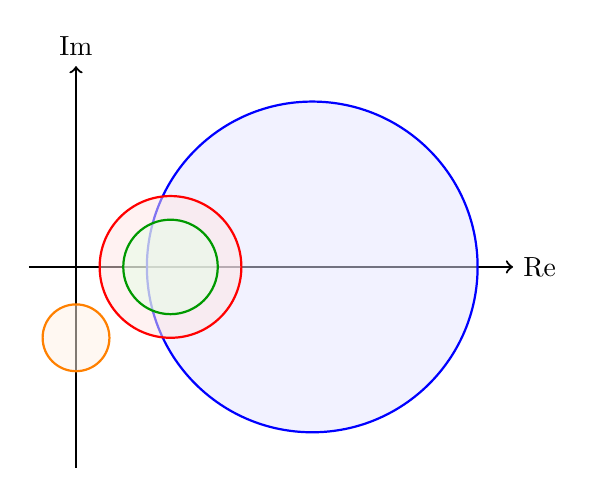
\begin{tikzpicture}[scale=0.3]
            \draw[->, thick] (-2,0) -- (18.5,0) node[right] {Re};
            \draw[->, thick] (0,-8.5) -- (0,8.5) node[above] {Im};

            \draw[blue, thick, fill=blue!10, fill opacity=0.5] (10,0) circle (7);
            \draw[red, thick, fill=red!10, fill opacity=0.5] (4,0) circle (3);
            \draw[green!60!black, thick, fill=green!10, fill opacity=0.5] (4,0) circle (2);
            \draw[orange, thick, fill=orange!10, fill opacity=0.5] (0,-3) circle (1.414);
        \end{tikzpicture}
        \end{center}
        \vspace{-3cm}
    \end{wrapfigure}
    Consideriamo la matrice
    \[
        \begin{pmatrix}
            10 & 1 & 3 & 3 \\
            -1 & 4 & 0 & 1 \\
            i & i & 4 & i \\
            i+1 & 0 & 0 & 3i
        \end{pmatrix}
    \]
    Abbiamo i seguenti cerchi di Gershgorin
    \begin{align*}
        C_1 &= \{ z \in \complexnumbers \suchthat |z-10| \leq 7\} \\
        C_2 &= \{ z \in \complexnumbers \suchthat |z-4| \leq 2\} \\
        C_3 &= \{ z \in \complexnumbers \suchthat |z-4| \leq 3\} \\
        C_4 &= \{ z \in \complexnumbers \suchthat |z-3i| \leq \sqrt{2}\}
    \end{align*}
    Possiamo notare che sicuramente il determinante della matrice non è nullo.
    \wrapfill
\end{snippetexample}

\begin{snippetexample}{gershgorin-theorem-example-2}{Teorema di Gershgorin II e III}
    \begin{wrapfigure}{r}{8cm}
        \begin{center}
            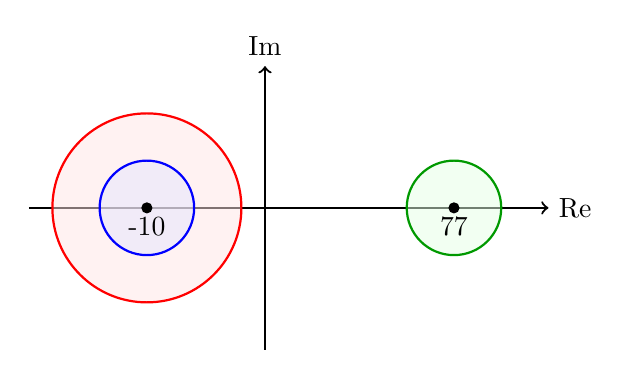
\begin{tikzpicture}[scale=0.6]
            \draw[->, thick] (-5,0) -- (6,0) node[right] {Re};
            \draw[->, thick] (0,-3) -- (0,3) node[above] {Im};

            \draw[red, thick, fill=red!10, fill opacity=0.5] (-2.5,0) circle (2);
            \draw[blue, thick, fill=blue!10, fill opacity=0.5] (-2.5,0) circle (1);

            \draw[green!60!black, thick, fill=green!10, fill opacity=0.5] (4,0) circle (1);

            \filldraw[black] (-2.5,0) circle (3pt) node[below] {-10};
            \filldraw[black] (4,0) circle (3pt) node[below] {77};
            \end{tikzpicture}
        \end{center}
        \vspace{-3cm}
    \end{wrapfigure}
    Consideriamo la matrice \[
        A = \begin{pmatrix}
            -10 & 1   &     &     &                &    \\
            1   & -10 & 1   &     & \text{\huge 0} &    \\
                & 1   & -10 & 1   &                &    \\
                &     & 1   & -10 & 1              &    \\
                & \text{\huge 0} && 1        & -10 & 1  \\
                &     &     &     & -1             & 77 
        \end{pmatrix}
    \]
    Mostrare che esiste un autovalore \(\lambda\) di questa matrice tale che
    \(\lambda = \rho(A)\). \\
    Abbiamo i cerchi
        \begin{align*}
        C_1 &= \{ z \in \complexnumbers \suchthat |z+10| \leq 1\} \\
        C_2 = C_3 = C_4 = C_5 &= \{ z \in \complexnumbers \suchthat |z+10| \leq 2\} \\
        C_6 &= \{ z \in \complexnumbers \suchthat |z-77| \leq 1\}
    \end{align*}
    C'è quindi un singolo autovalore in \(C_6\),
    ma quest'ultimo non può essere propriamente complesso in quanto ci sarebbe un'altro
    autovalore coniugato nello stesso cerchio.
    Quindi quell'autovalore è reale e coincide con il raggio spettrale, data la sua distanza dall'origine.
    Il suo grafo associato è fortemente connesso:
    \begin{center}
        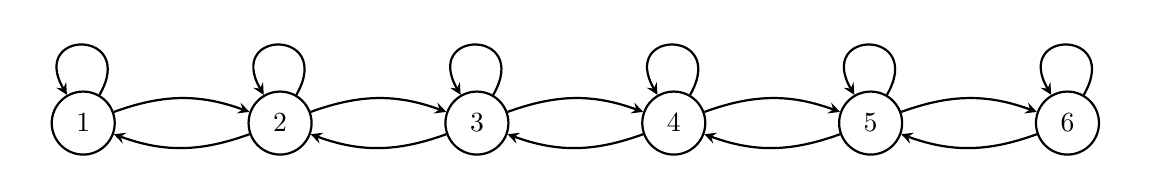
\begin{tikzpicture}[>=stealth, node distance=2cm]
            \node[circle, draw, thick, minimum size=8mm] (1) at (0,0) {1};
            \node[circle, draw, thick, minimum size=8mm] (2) at (2.5,0) {2};
            \node[circle, draw, thick, minimum size=8mm] (3) at (5,0) {3};
            \node[circle, draw, thick, minimum size=8mm] (4) at (7.5,0) {4};
            \node[circle, draw, thick, minimum size=8mm] (5) at (10,0) {5};
            \node[circle, draw, thick, minimum size=8mm] (6) at (12.5,0) {6};

            \foreach \i in {1,2,3,4,5,6} {
                \draw[->, thick] (\i) to[out=60, in=120, looseness=6] (\i);
            }

            \foreach \i/\j in {1/2, 2/3, 3/4, 4/5, 5/6} {
                \draw[->, thick] (\i) to[bend left=20] (\j);
                \draw[->, thick] (\j) to[bend left=20] (\i);
            }
        \end{tikzpicture}
    \end{center}
    \wrapfill
\end{snippetexample}

\end{document}